\section{N-Back} \label{sec:impl/tasks}
\subsection{Overview}

Section \ref{sec:bt/cognitive_impacts} listed a number of standard experiments that are known to produce some form of mental strain on the subject. These experiments have all been used extensively in many fields of research, so their effects on the subjects are constant and familiar. Therefore, they may be considered a sufficient proxy for cognitive load for the purposes of this thesis. We will employ the N-Back task. It was chosen primarily for its distinct levels of difficulty, which could be directly translated to levels of cognitive load for classification. Besides, it is simple in nature, straightforward to implement, and requires nothing but a stimulus screen and an input device to deploy. 

The N-Back task operates by displaying a series of stimulus in the form of single letters on screen, switching stimulus every other second. For each stimuli, the subject is asked to indicate by a key press whether the presented stimulus is the same as the one presented N screens before. Naturally, task difficulty increases with increasing N, demanding more and more information to be kept in working memory at any one time. To perform well, the subject must constantly allocate attention to the task. Multiple studies have shown that both pupil diameter and \acrshort{ebr} increases with increasing N \cite{hopstaken2015, belayachi2015, brouwer2014, niezgoda2015}, proving its relevance for cognitive load classification. 

\subsection{Details}

For this particular use case, the author chose three difficulty levels; N=0, N=1, and N=2. Many related experiments also employ N=3. However, experience shows that most participants tend to find this level too difficult and give up early \cite{ayaz2007, izzetoglu2007}. Additionally, since this thesis merely aims to classify distinct levels of cognitive load, three levels would be more than sufficient.

The first level (N=0) is intended to impose no particular cognitive load on the subject besides requiring sustained attention. It is achieved by showing the target stimulus before the task commences. This way, working memory merely needs to memorize one constant target. For levels N=1 and N=2, the target stimuli is dynamically determined by the N-back stimuli.

Experimental trials are structured so that the subject is exposed to continuous engagement for only five minutes at a time. Every trial consists of three N-Back blocks, each split into three block segments for every task difficulty (N=0, N=1, N=2). Block segments are further structured as illustrated in figure \ref{fig:impl_NBackBlockSeg}. In this particular example, N=1. It begins with two milliseconds of segment presentation, where the subject is made aware of the segment difficulty. Then, nine series of screens are presented, each showing a stimulus for 500 milliseconds, followed by a 1500 milliseconds long blank screen. Finally, a fixation cross is presented for 6000 milliseconds. The idle, onset, execution, and offset labels in the figure will be detailed in section \ref{sec:impl/dataset}.

% The target stays constant throughout the task, such that the subject does not need to engage working memory besides , having a constant target throughout the trial.

\begin{figure}[h]
    \centering
    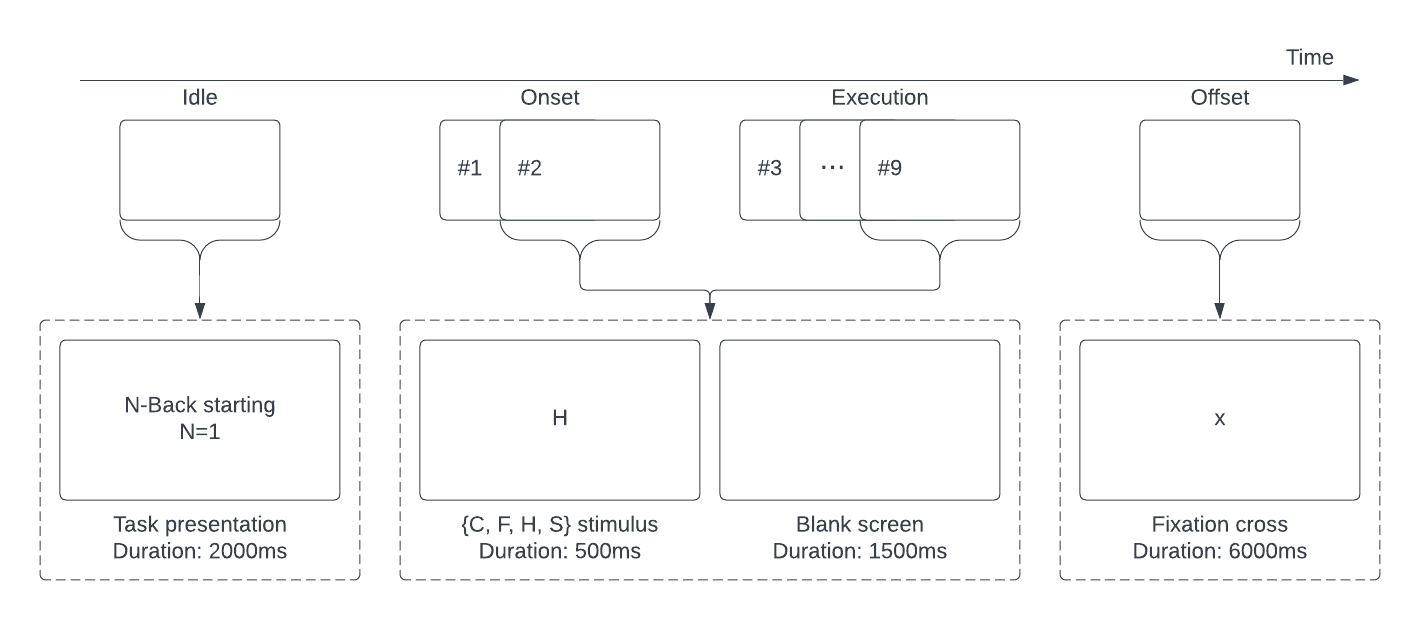
\includegraphics[width=0.8\textwidth]{figures/impl_NBackBlock.png}
    \caption{Timeline for each N-Back block segment. The current example represents N=0. One N-Back block represents three such block segments, one for each difficulty level.}
    \label{fig:impl_NBackBlockSeg}
\end{figure}


